% Lesson 3. Compile from the repo root via main.tex.
% Theme: lesson 1 preamble, with the lesson 2 overrides.
% Wording is the 20 Nov 2026 deck. Only the frame chrome changes.
% Lesson 2 theme: Lesson 1 preamble, then three overrides.
% =============================================================
% Agentic AI for Economic Research, Lesson 1 theme (v2)
% Compiler: pdflatex (no fontspec). Paths are relative to repo root.
% Design read: lecture deck for economics PhD students and faculty,
% watched over a screen share; calm academic language; one ink colour,
% one accent, real screenshots and data charts as the only visuals.
% Dials: variance 5, motion 1, density 4.
% =============================================================

\documentclass[aspectratio=169,10pt]{beamer}

\usepackage[T1]{fontenc}
\usepackage[utf8]{inputenc}
\usepackage[english]{babel}

\usepackage[default,scale=0.95]{sourcesanspro}
\usepackage[scaled=0.85]{sourcecodepro}
\renewcommand{\familydefault}{\sfdefault}
\usepackage{microtype}

\usepackage{graphicx}
\usepackage{xcolor}
\newcommand{\rev}[1]{#1}
\usepackage{tikz}
\usetikzlibrary{positioning,arrows.meta,calc,fit,backgrounds}
\usepackage{pgfplots}
\usepackage{pgfplotstable}
\pgfplotsset{compat=1.18}
\usepgfplotslibrary{dateplot}
\usepackage{tabularx}
\usepackage{booktabs}
\usepackage{array}
\usepackage{ragged2e}
\usepackage{hyperref}
\usepackage[most]{tcolorbox}
\usepackage{fancyvrb}
\usepackage[round,authoryear]{natbib}
\bibliographystyle{plainnat}

\ifdefined\DeclareUnicodeCharacter
  \DeclareUnicodeCharacter{2192}{\ensuremath{\rightarrow}}
  \DeclareUnicodeCharacter{2190}{\ensuremath{\leftarrow}}
  \DeclareUnicodeCharacter{2717}{x}
  \DeclareUnicodeCharacter{00B7}{\textperiodcentered}
\fi

\graphicspath{{assets/lesson1/screens/}{assets/lesson1/logos/}{assets/covers/}{assets/real/}}

% One cover. Same band, same fonts, same lines. \coverframe{image}{title}{subtitle}{n}
\newcommand{\coverframe}[4]{%
\begin{frame}[plain]
  \begin{tikzpicture}[remember picture,overlay]
    \node[anchor=center,inner sep=0] at (current page.center)
      {\includegraphics[width=\paperwidth,height=\paperheight]{#1}};
    \fill[black,opacity=.55] (current page.south west) rectangle ($(current page.south west)+(\paperwidth,3.45cm)$);
    \node[anchor=south west,text width=13.4cm,align=left,inner sep=0pt] at ($(current page.south west)+(0.7cm,0.38cm)$)
      {{\color{white}\fontsize{25}{29}\selectfont\bfseries #2}\\[4pt]
       {\normalsize\color{white!85} #3}\\[5pt]
       {\footnotesize\color{white!78} Agentic AI for Economic Research \quad|\quad Lesson #4 \quad|\quad Marco Le Moglie}\\[4pt]
       {\hypersetup{urlcolor=white!85}\href{https://github.com/MarcoLeMoglie/Agentic_Economic_Research}{\footnotesize\color{white!85}
\includegraphics[height=1.05em]{github_mark_white.png}\ GitHub repo}}};
  \end{tikzpicture}
\end{frame}}

% ---------- Palette (locked: one ink, one accent, one cool grey family) ----------
\definecolor{ink}{HTML}{163A59}
\definecolor{accent}{HTML}{D97706}
\definecolor{dark}{HTML}{111827}
\definecolor{muted}{HTML}{4B5563}
\definecolor{faint}{HTML}{9CA3AF}
\definecolor{hair}{HTML}{D1D5DB}
\definecolor{paper}{HTML}{F8FAFC}
\definecolor{tint}{HTML}{EEF2F6}
% semantic only (good / bad), never decorative
\definecolor{good}{HTML}{166534}
\definecolor{bad}{HTML}{B91C1C}
\definecolor{stepR}{HTML}{6D28D9}
\definecolor{stepE}{HTML}{0F766E}

\hypersetup{colorlinks=true,linkcolor=ink,urlcolor=ink,citecolor=ink}

% ---------- Beamer base ----------
\useinnertheme{rectangles}
\useoutertheme{default}
\setbeamersize{text margin left=2.2em,text margin right=2.2em}
\setbeamercolor{background canvas}{bg=paper}
\setbeamercolor{normal text}{fg=dark}
\setbeamercolor{structure}{fg=ink}
\setbeamercolor{alerted text}{fg=accent}
\setbeamertemplate{navigation symbols}{}

\setbeamerfont{frametitle}{size=\Large,series=\bfseries}
\setbeamercolor{frametitle}{fg=ink}
\setbeamertemplate{frametitle}{%
  \vspace{0.9em}%
  \begin{minipage}[t]{\dimexpr\paperwidth-4.4em\relax}%
    \raggedright\insertframetitle\par
    \vspace{-0.35em}{\color{accent}\rule{2.2em}{1.2pt}}%
  \end{minipage}%
  \vspace{0.2em}%
}

\setbeamertemplate{footline}{%
  \leavevmode\hbox to \paperwidth{%
    \hspace{2.2em}{\color{faint}\fontsize{6.5}{8}\selectfont Agentic AI for Economic Research, Lesson 1}%
    \hfill{\color{faint}\fontsize{6.5}{8}\selectfont\insertframenumber}\hspace{2.2em}}%
  \vspace{0.9em}%
}

% bullets: small grey square, no chevrons
\setbeamertemplate{itemize item}{\raisebox{0.18em}{\color{faint}\rule{0.32em}{0.32em}}}
\setbeamertemplate{itemize subitem}{\raisebox{0.2em}{\color{hair}\rule{0.26em}{0.26em}}}
\setbeamertemplate{enumerate item}{\color{ink}\bfseries\insertenumlabel.}
\setlength{\leftmargini}{1.1em}

% ---------- tcolorbox styles (radius locked at 2pt) ----------
\tcbset{
  l1base/.style={enhanced,arc=2pt,outer arc=2pt,boxrule=0pt,
    left=0pt,right=0pt,top=0pt,bottom=0pt},
}

% Definition: accent rule on the left, term, text, source
\newtcolorbox{defbox}[1]{enhanced,frame hidden,interior hidden,
  borderline west={1.6pt}{0pt}{accent},
  left=0.9em,right=0pt,top=0.15em,bottom=0.15em,
  fontupper=\normalsize,
  before upper={{\color{ink}\bfseries #1}\par\vspace{0.25em}}}
\newcommand{\defn}[3]{%
  \begin{defbox}{#1}#2\if\relax\detokenize{#3}\relax\else\par\vspace{0.3em}{\color{muted}\scriptsize #3}\fi\end{defbox}}

% Real file or real terminal output, read verbatim from disk:
% \filebox[width]{path}{caption}
\newcommand{\filebox}[3][\linewidth]{%
  \begin{tcolorbox}[l1base,width=#1,colback=white,
      borderline={0.4pt}{0pt}{hair},left=0.6em,right=0.4em,top=0.4em,bottom=0.4em]
    \VerbatimInput[fontsize=\fontsize{6}{7.1}\selectfont,formatcom=\color{dark}]{#2}%
  \end{tcolorbox}%
  \par\vspace{0.15em}{\color{muted}\scriptsize #3}}

% Screenshot frame: hairline border, caption below
\newcommand{\shot}[3][\linewidth]{%
  \begin{tcolorbox}[l1base,width=#1,colback=white,
      borderline={0.4pt}{0pt}{hair},left=0pt,right=0pt,top=0pt,bottom=0pt]
    \includegraphics[width=\linewidth]{#2}%
  \end{tcolorbox}%
  \par\vspace{0.15em}{\color{muted}\scriptsize #3}}
\newcommand{\shoth}[4][\linewidth]{% height-capped variant: [width]{file}{height}{caption}
  \begin{tcolorbox}[l1base,width=#1,colback=white,halign=center,
      borderline={0.4pt}{0pt}{hair},left=0pt,right=0pt,top=0pt,bottom=0pt]
    \includegraphics[width=\linewidth,height=#3,keepaspectratio]{#2}%
  \end{tcolorbox}%
  \par\vspace{0.15em}{\color{muted}\scriptsize #4}}

% Source line at the bottom of a frame
\newcommand{\source}[1]{\vfill{\color{muted}\scriptsize Source: #1\par}}

% One statement per slide, at most
\newcommand{\takeaway}[1]{\par\vspace{0.5em}{\color{ink}\large\bfseries #1\par}}

% Small group label used instead of numbered labels
\newcommand{\group}[1]{{\color{ink}\bfseries #1}\par\vspace{0.2em}}

% Section divider: ink background, topic name only
\newcommand{\sectionframe}[2][]{%
\begin{frame}[plain]
  \begin{tikzpicture}[remember picture,overlay]
    \fill[ink] (current page.south west) rectangle (current page.north east);
    \node[anchor=south west,inner sep=0pt,text=white,align=left,text width=0.8\paperwidth]
      at ($(current page.south west)+(1.6cm,1.7cm)$)
      {{\fontsize{28}{33}\selectfont\bfseries #2}\par\vspace{0.4em}{\color{white!75!ink}\large #1}};
    \fill[accent] ($(current page.south west)+(1.6cm,1.25cm)$) rectangle ++(1.4cm,0.06cm);
  \end{tikzpicture}
\end{frame}}

% Live demo placeholder
\newcommand{\demoframe}[3]{% {title}{what we do}{what to look at}
\begin{frame}{#1}
  \begin{columns}[T,onlytextwidth]
    \column{0.55\textwidth}
      \group{What we do}
      #2
    \column{0.40\textwidth}
      \group{What to look at}
      #3
  \end{columns}
\end{frame}}

% ---------- TikZ styles ----------
\tikzset{
  lab/.style={align=center,font=\small,text=dark},
  sub/.style={align=center,font=\scriptsize,text=muted},
  hl/.style={align=center,font=\small\bfseries,text=ink},
  frameb/.style={draw=hair,line width=0.5pt,rounded corners=2pt,fill=white},
  inkb/.style={draw=ink,line width=0.8pt,rounded corners=2pt,fill=white},
  accb/.style={draw=accent,line width=0.9pt,rounded corners=2pt,fill=white},
  arr/.style={-{Stealth[length=4pt]},line width=0.6pt,color=faint},
  arrA/.style={-{Stealth[length=5pt]},line width=0.9pt,color=accent},
}

% ---------- pgfplots defaults: no legends, no background tracks ----------
\pgfplotsset{
  l1axis/.style={
    axis lines*=left,
    axis line style={hair},
    tick style={draw=none},
    ticklabel style={font=\scriptsize,color=muted},
    label style={font=\scriptsize,color=muted},
    every axis plot/.append style={line width=0.6pt},
    enlargelimits=false,
    clip=false,
    /pgf/number format/assume math mode=true,
  },
  % keep only rows whose column #1 equals #2 (colour bars by group from the CSV)
  only if/.style 2 args={
    x filter/.code={\getthisrow{#1}\tempa\edef\tempb{#2}%
      \ifx\tempa\tempb\else\def\pgfmathresult{inf}\fi}},
}

% ---------- Metadata ----------
\title{Agentic AI for Economic Research}
\author{Marco Le Moglie}
\institute{Catholic University of the Sacred Heart}


\setbeamertemplate{footline}{%
  \leavevmode\hbox to \paperwidth{%
    \hfill{\color{faint}\fontsize{6.5}{8}\selectfont\insertframenumber}\hspace{2.2em}}%
  \vspace{0.9em}%
}

\graphicspath{{assets/lesson2/screens/}{assets/lesson2/illustrations/}{assets/lesson2/diagrams/}{assets/lesson1/logos/}{assets/real/}}

% Macros used by the Lesson 2 source pack. Colours and frame chrome stay on the Lesson 1 theme.
\ifdefined\DeclareUnicodeCharacter
  \DeclareUnicodeCharacter{2013}{--}
  \DeclareUnicodeCharacter{2014}{---}
  \DeclareUnicodeCharacter{2018}{`}
  \DeclareUnicodeCharacter{2019}{'}
  \DeclareUnicodeCharacter{201C}{``}
  \DeclareUnicodeCharacter{201D}{''}
\fi
% Review colour accepted: \chg keeps the words and no longer paints them.
\newcommand{\chg}[1]{#1}
\newcommand{\chgshoth}[4][\linewidth]{%
  \begin{tcolorbox}[l1base,width=#1,colback=white,halign=center,
      borderline={1pt}{0pt}{hair},left=0pt,right=0pt,top=0pt,bottom=0pt]
    \includegraphics[width=\linewidth,height=#3,keepaspectratio]{#2}%
  \end{tcolorbox}%
  \par\vspace{0.15em}{\color{muted}\scriptsize #4}}
\newtcolorbox{chgfig}{l1base,colback=paper,borderline={1pt}{0pt}{hair},left=4pt,right=4pt,top=4pt,bottom=4pt,halign=center}

% YouTube clip card: \ytclip{video id}{title}{description}; thumbnail in assets/lesson2/video/yt-<id>.jpg
\newcommand{\ytclip}[3]{%
  \begin{minipage}[t]{5.15cm}
    \centering
    \href{https://www.youtube.com/watch?v=#1}{%
      \begin{tikzpicture}
        \node[inner sep=0pt] (img) {\includegraphics[height=3.35cm]{assets/lesson2/video/yt-#1.jpg}};
        \draw[hair,line width=1pt] (img.south west) rectangle (img.north east);
        \fill[black,opacity=.55] (img.center) circle (0.42cm);
        \fill[white] ($(img.center)+(-0.13,-0.2)$) -- ($(img.center)+(-0.13,0.2)$) -- ($(img.center)+(0.21,0)$) -- cycle;
      \end{tikzpicture}}\par\vspace{0.35em}
    {\color{ink}\small\bfseries #2}\par\vspace{0.1em}
    {\color{muted}\scriptsize #3}
  \end{minipage}}

\newcommand{\kicker}[1]{}
\newcommand{\subt}[1]{{\color{muted}\small #1}\par\vspace{.65em}}
\newcommand{\tagline}[1]{\takeaway{#1}}
\newcommand{\citefoot}[1]{}
\newcommand{\boxtitle}[1]{{\color{ink}\bfseries #1}}
\tcbset{l2base/.style={enhanced,arc=2pt,outer arc=2pt,boxrule=0.55pt,colframe=hair,colback=white,left=2mm,right=2mm,top=1.5mm,bottom=1.5mm}}
\newcommand{\coursebox}[2]{\begin{tcolorbox}[l2base]\boxtitle{#1}\par\vspace{1mm}{\small #2}\end{tcolorbox}}
\newcommand{\sboxblue}[2]{\begin{tcolorbox}[l2base,colback=tint,colframe=ink!24]\boxtitle{#1}\par\vspace{1mm}{\small #2}\end{tcolorbox}}
\newcommand{\lightimg}[2]{\begin{tcolorbox}[l2base,left=0pt,right=0pt,top=0pt,bottom=0pt]\includegraphics[width=\linewidth,height=#2,keepaspectratio]{#1}\end{tcolorbox}}
\newcommand{\inlinecode}[1]{{\ttfamily\small\color{ink}#1}}
\newcommand{\lc}[1]{{\color{muted}\footnotesize #1}}
\tikzset{
  lbox/.style={draw=hair,rounded corners=2pt,fill=white,text width=2.35cm,align=center,inner sep=8pt,font=\small},
  lblue/.style={draw=ink,rounded corners=2pt,fill=tint,text width=2.35cm,align=center,inner sep=8pt,font=\small},
  larrow/.style={-{Stealth[length=5pt]},draw=ink,line width=.8pt}
}

\renewcommand{\demoframe}[3]{%
\begin{frame}{#1}
  \begin{columns}[T,onlytextwidth]
    \column{0.55\textwidth}
      \group{What we do}
      #2
    \column{0.40\textwidth}
      \group{What to look at}
      #3
  \end{columns}
\end{frame}}


\setbeamertemplate{footline}{%
  \leavevmode\hbox to \paperwidth{%
    \hspace{2.2em}{\color{faint}\fontsize{6.5}{8}\selectfont Agentic AI for Economic Research, Lesson 3}%
    \hfill{\color{faint}\fontsize{6.5}{8}\selectfont\insertframenumber}\hspace{2.2em}}%
  \vspace{0.9em}%
}
\graphicspath{{assets/lesson1/logos/}{assets/covers/}{assets/lesson3/tex/}{assets/real/}}
\renewcommand{\takeaway}[1]{\par\vspace{1.55em}{\color{ink}\large\bfseries #1\par}}

\begin{document}

\coverframe{assets/covers/03_automations_control_background.jpg}{Automations \& Control}{Designing and reviewing agent workflows}{3}

\begin{frame}{Today: Automations and Control}
\subt{Two different problems in a research workflow.}
\begin{columns}[T,onlytextwidth]
\column{0.48\textwidth}
\begin{tcolorbox}[l2base,colback=tint,colframe=ink!24,height=2.85cm,valign=top]
\boxtitle{Automations}\par\vspace{1mm}{\small
\textbf{When does work start?}\\[0.35em]
A scheduled run, an event or a verified condition.\\[0.45em]
A script or an agent completes a defined task.}
\end{tcolorbox}
\column{0.48\textwidth}
\begin{tcolorbox}[l2base,height=2.85cm,valign=top]
\boxtitle{Control}\par\vspace{1mm}{\small
\textbf{How do we inspect the work?}\\[0.35em]
Check facts and sources, not only whether code ran.\\[0.45em]
Expose hallucinations, unsupported claims and sloppy outputs.}
\end{tcolorbox}
\end{columns}
\takeaway{The researcher defines both the allowed actions and how to review their consequences.}
\end{frame}

\sectionframe{Automations}

\begin{frame}{Research tasks with repeatable triggers}
\subt{Examples across a conventional empirical paper.}
\begin{itemize}\setlength{\itemsep}{0.55em}
\item \textbf{Literature.} Weekly retrieval of new papers; report titles, DOI and relevance.
\item \textbf{Data.} Check whether the source published a new release or revised a codebook.
\item \textbf{Code.} Re-run tests when the analysis script or input dataset changes.
\item \textbf{Results.} Rebuild tables after a validated data update; compare with baseline.
\end{itemize}
\end{frame}

\begin{frame}{Three kinds of triggers}
\subt{Each trigger can start a deterministic script or an agentic workflow.}
\begin{itemize}\setlength{\itemsep}{0.7em}
\item \textbf{Scheduled.} Monday at 09:00: search for working papers added during the previous week.
\item \textbf{Event-driven.} A new Stata do-file is saved by an agent: run the project validator.
\item \textbf{Condition-driven.} A bulk data job becomes READY: download, validate and import its output.
\end{itemize}
\end{frame}

\begin{frame}{Where an event can originate}
\subt{Different mechanisms expose different events.}
\begin{itemize}\setlength{\itemsep}{0.45em}
\item \textbf{Agent hook.} A tool writes a \texttt{.do} file; a registered hook checks the edited code.
\item \textbf{File watcher.} A CSV appears in an incoming folder; a watcher starts validation.
\item \textbf{Webhook.} A data service sends a completion notice for a submitted job.
\item \textbf{Repository event.} A remote commit starts the project test suite.
\end{itemize}
\takeaway{Use the event source that corresponds to the process being monitored.}
\end{frame}

\begin{frame}{Where an automation actually runs}
\begin{columns}[T,onlytextwidth]
\column{0.48\textwidth}
\begin{tcolorbox}[l2base,colback=tint,colframe=ink!24,height=2.15cm,valign=top]
\boxtitle{Self-managed host}\par\vspace{1mm}{\small
\textbf{Laptop, Mac mini or VPS}\\[0.35em]
Runs while that machine is on and reachable.}
\end{tcolorbox}
\column{0.48\textwidth}
\begin{tcolorbox}[l2base,height=2.15cm,valign=top]
\boxtitle{Provider-managed computer}\par\vspace{1mm}{\small
\textbf{Grok Bot / Muse / OpenClaw}\\[0.35em]
Can continue independently of your laptop.}
\end{tcolorbox}
\end{columns}
\takeaway{On your own machine, the run stops if that computer is off. That is not true for Grok Bot, Muse or OpenClaw.}
\end{frame}

\begin{frame}{Decide the agent’s permissions beforehand}
\subt{Unattended processes should use narrow credentials and approval gates.}
\begin{itemize}\setlength{\itemsep}{0.55em}
\item \textbf{Can run automatically.} Read public metadata; create logs; validate candidates; report differences.
\item \textbf{Needs review.} Replace baseline data; change a sample definition; edit final estimates.
\item \textbf{Requires explicit approval.} Publish findings; send external messages; access restricted data; spend above budget.
\end{itemize}
\takeaway{Before you approve, look at the input, the change the agent proposes, the diff, the tests, and where the result will be written.}
\end{frame}

\begin{frame}{An automation already used in research}
\begin{columns}[T,onlytextwidth]
\column{0.48\textwidth}
\begin{itemize}\setlength{\itemsep}{0.38em}
\item \textbf{Harvest.} Collect candidate papers from the configured sources and save the shortlist.
\item \textbf{Review.} Inspect the editorial dashboard and flag accepted items.
\item \textbf{Render.} Generate the issue only when the review gate is satisfied.
\item \textbf{Send.} An approved campaign is sent only after an explicit release decision.
\end{itemize}
\column{0.50\textwidth}
\vspace{0.15em}

\includegraphics[width=\linewidth]{assets/lesson3/tex/newsletter_assist.jpg}
\end{columns}
\end{frame}

\sectionframe{Control}

\begin{frame}{The researcher becomes a middle manager}
\subt{Several agents can research, code, revise and check files while you handle other work.}
\group{The problem}
How can you tell whether they used the correct data, followed the agreed design and reported truthful results?
\takeaway{Control is not a magic PASS/FAIL test. Design workflows so mistakes are visible and cheap to investigate.}
\end{frame}

\begin{frame}{What can go wrong with an AI agent?}
\begin{itemize}\setlength{\itemsep}{0.35em}
\item \textbf{Hallucination.} Invented citations, unsupported numbers or variables.
\item \textbf{Context rot.} Earlier constraints are lost in a long working session.
\item \textbf{Reward hacking.} A check passes while the actual research goal is missed.
\item \textbf{Sycophancy.} The agent agrees with a mistaken premise.
\item \textbf{Automation bias.} The researcher trusts an output without inspecting its evidence.
\item \textbf{Model drift.} A changed model produces different behavior on the same task.
\end{itemize}
\end{frame}

\begin{frame}{Review follows the researcher’s expertise}
\subt{Choose tests that you can interpret and maintain.}
\begin{itemize}\setlength{\itemsep}{0.42em}
\item \textbf{Econometric design.} Identification, units, outcome definition, standard errors, sensitivity.
\item \textbf{Data expertise.} Coverage, sources, variable construction, revised classifications.
\item \textbf{Programming.} Tests, dependency versions, reproducibility, unintended file writes.
\item \textbf{Academic writing.} Claims, evidence, references, interpretation and omissions.
\end{itemize}
\takeaway{Start with checks that match your strongest competencies; add tools where you need visibility.}
\end{frame}

\begin{frame}{A reviewable plan comes before execution}
\begin{itemize}\setlength{\itemsep}{0.5em}
\item \textbf{Question + unit.} Effect of a local program on municipal employment; municipality-year panel.
\item \textbf{Design + sample.} Difference-in-differences; treated and eligible comparison municipalities.
\item \textbf{Fixed decisions.} Treatment date, outcome, controls, weights and standard-error strategy.
\item \textbf{Required diagnostics.} Pre-trends, missingness, spillovers, alternate samples, placebo dates.
\end{itemize}
\takeaway{The agent should record proposed departures from the plan and request approval.}
\end{frame}

\begin{frame}{Five ways to make agent work easier to inspect}
\begin{itemize}\setlength{\itemsep}{0.42em}
\item \textbf{Familiar code.} Use the Stata, R or Python conventions you already follow.
\item \textbf{Run report.} List changes, failed tests and unresolved questions.
\item \textbf{Side-by-side check.} Put the source record next to the value the agent took from it.
\item \textbf{Second opinion.} Give a critic agent a separate audit assignment.
\item \textbf{Project Brain.} Record decisions and the evidence supporting them.
\end{itemize}
\end{frame}

\begin{frame}[fragile]{Ask the agent to code in your style}
\subt{Short Stata blocks, explicit comments and checks you can inspect.}
\begin{columns}[T,onlytextwidth]
\column{0.58\textwidth}
\begin{tcblisting}{l2base,listing only,left=1.4mm,right=1.2mm,top=1mm,bottom=1mm,
  listing options={basicstyle=\ttfamily\fontsize{6.2}{7.4}\selectfont,breaklines=true,columns=fullflexible}}
* Make a log before touching the dataset
capture log close
log using "logs/check_sample.log", replace text
use "data/candidate_panel.dta", clear
isid municipality year
* Apply the agreed analysis period
keep if inrange(year, 2015, 2026)
* Verify variables and inspect the sample
assert !missing(outcome, treatment)
count
log close
\end{tcblisting}
\column{0.38\textwidth}
\group{Instructions to the agent}
\begin{itemize}\setlength{\itemsep}{0.45em}
\item Match my existing do-files.
\item Use clear variables and comments.
\item Avoid unnecessary programs or loops.
\item Do not change the research sample silently.
\end{itemize}
\end{columns}
\end{frame}

\begin{frame}{A report that identifies the items requiring review}
\subt{The agent should point to evidence, not simply state that the task is finished.}
\begin{columns}[T,onlytextwidth]
\column{0.58\textwidth}
\group{Report after a run (illustrative)}
\begin{itemize}\setlength{\itemsep}{0.38em}
\item \textbf{Files.} \texttt{analysis.do}, \texttt{panel\_build.do}
\item \textbf{Data.} 18 municipalities revised
\item \textbf{Checks.} Unique key: PASS / Missing outcome: PASS
\item \textbf{Estimate.} 0.14 → 0.11
\item \textbf{Question.} Why did the sample lose 37 observations?
\end{itemize}
\column{0.38\textwidth}
\group{What to inspect}
\begin{itemize}\setlength{\itemsep}{0.38em}
\item Code diff
\item Source revision
\item Sample change
\item Accepted specification
\end{itemize}
\end{columns}
\takeaway{Report the change and the file where it can be checked.}
\end{frame}

\begin{frame}{Use a second agent as a critic}
\subt{Specify exactly which agent makes the result and which agent checks it.}
\begin{columns}[T,onlytextwidth]
\column{0.48\textwidth}
\group{Working agent}
\begin{itemize}\setlength{\itemsep}{0.4em}
\item Estimates the DID model
\item Writes code and results.
\item Lists chosen controls and timing.
\item Exports figures and tables.
\end{itemize}
\column{0.48\textwidth}
\group{Critic agent}
\begin{itemize}\setlength{\itemsep}{0.4em}
\item Challenges the conclusion
\item Checks pre-trends and timing.
\item Questions cluster level and sample.
\item Finds claims unsupported by tables.
\end{itemize}
\end{columns}
\takeaway{Give the critic independent instructions and access to evidence. The researcher evaluates disagreements.}
\end{frame}

\begin{frame}{Make checks run whenever an output changes}
\subt{An automation can also be the mechanism that makes scientific review easier.}
\begin{itemize}\setlength{\itemsep}{0.5em}
\item \textbf{When.} An agent updates a table or figure.
\item \textbf{Check.} Compare its sample, estimates and captions with the current paper text.
\item \textbf{Report.} List each disagreement with the file and line or table reference.
\item \textbf{Stop.} Do not replace accepted outputs until the researcher resolves the differences.
\end{itemize}
\takeaway{This check can run after an output event. The comparison may use scripts plus a dedicated reviewing agent.}
\end{frame}

\begin{frame}{PURGE: a dashboard for checking OCR}
\subt{A research interface built to let a human correct extracted historical data.}
\vspace{0.15em}
\begin{columns}[T,onlytextwidth]
\column{0.49\textwidth}
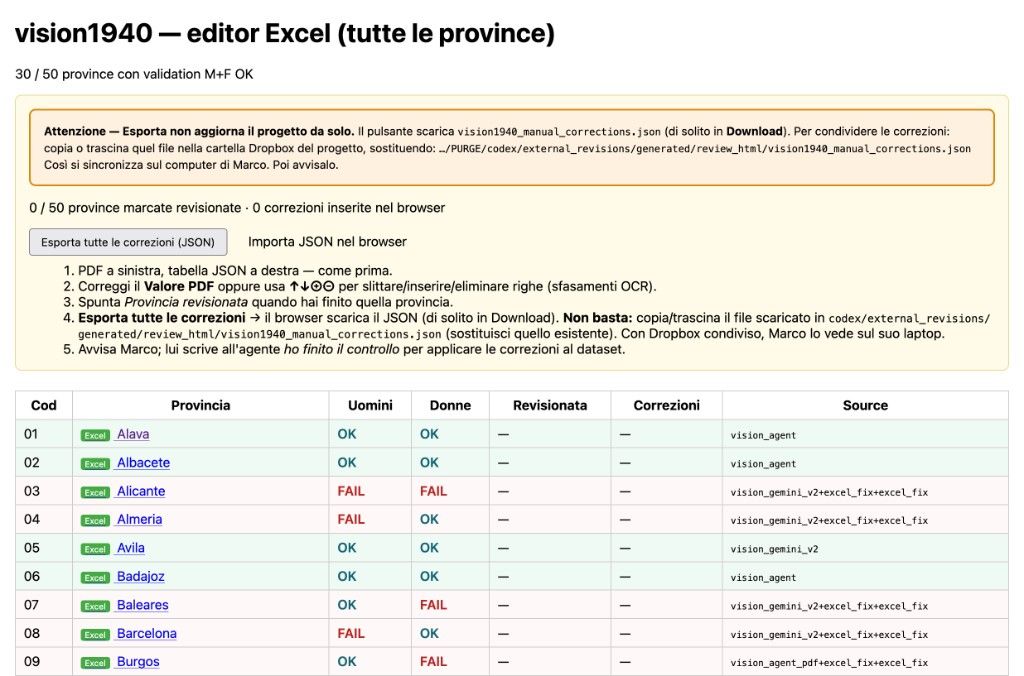
\includegraphics[width=\linewidth]{assets/lesson3/tex/purge_vision1940.png}
\column{0.49\textwidth}
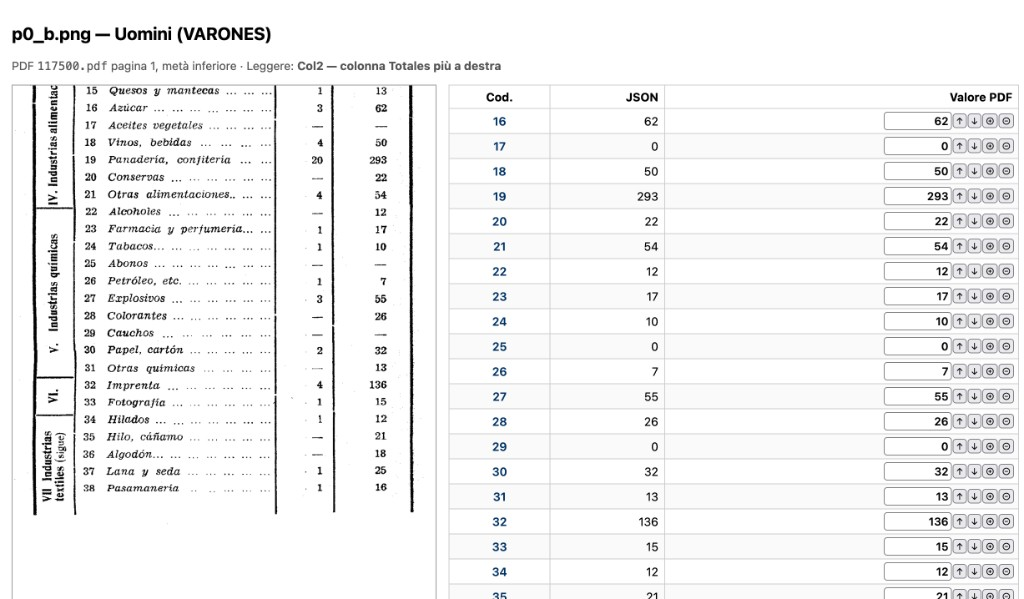
\includegraphics[width=\linewidth]{assets/lesson3/tex/purge_row_check.png}
\end{columns}
\end{frame}

\begin{frame}{What the PURGE interface lets you verify}
\subt{PDF on the left, extracted numbers on the right; only reviewed corrections move forward.}
\begin{itemize}\setlength{\itemsep}{0.32em}
\item \textbf{Source.} Open the original scanned 1940 census PDF.
\item \textbf{Extracted value.} Compare the cell from OCR/vision with the printed number.
\item \textbf{Correction.} Shift rows or replace the incorrect value manually.
\item \textbf{Review state.} Mark the province as reviewed and export corrections.
\item \textbf{Approval.} The export alone does not apply changes to the dataset.
\end{itemize}
\takeaway{This is control by interface design: the researcher sees the source, the extraction and the proposed correction.}
\end{frame}

\begin{frame}{The Second Brain as an LLM wiki}
\subt{Store decisions and evidence where another session can retrieve them.}
\begin{itemize}\setlength{\itemsep}{0.42em}
\item \texttt{*\_CURRENT\_STATE.md} --- Which dataset and analysis version are currently accepted?
\item \texttt{*\_DECISIONS.md} --- Which choices were made, when, by whom, and on what evidence?
\item \texttt{*\_NEXT\_ACTIONS.md} --- Which tasks are pending, blocked or awaiting approval?
\item \texttt{*\_LOG.md} --- What was executed, what changed, and where are the artifacts?
\end{itemize}
\takeaway{Useful retrieval: “What changed since the last accepted specification?”}
\end{frame}

\begin{frame}{Record the reason behind a methodological choice}
\subt{An example of a compact decision record, stored with the project.}
\begin{tcolorbox}[l2base]
{\ttfamily\small
\# Decision D-014 — 2026-11-19\\
Issue: Use municipality or province clustering?\\
Chosen: Province-level clustering + sensitivity.\\
Reason: Shared regional residual shocks.\\
Alternatives: Conley SE; municipality clusters.\\
Evidence: Residual correlation report, table E4.\\
Status: Accepted after independent review.\par}
\end{tcolorbox}
\takeaway{The Brain can recover this decision and its supporting evidence when a model, reviewer or agent asks about it.}
\end{frame}

\begin{frame}{Which line changed the sample?}
\subt{A small diff can be more useful than another generic dashboard.}
\begin{columns}[T,onlytextwidth]
\column{0.56\textwidth}
\group{One specific change}
\begin{tcolorbox}[l2base,left=1.6mm,right=1.4mm,top=1.2mm,bottom=1.2mm]
{\color{bad}\ttfamily\footnotesize - keep if inrange(year, 2017, 2026)}\\[0.25em]
{\color{good}\ttfamily\footnotesize + keep if inrange(year, 2015, 2026)}
\end{tcolorbox}
\vspace{0.6em}
Outcome: sample now includes two additional pre-treatment years.
\column{0.40\textwidth}
\group{Questions}
\begin{itemize}\setlength{\itemsep}{0.45em}
\item Who authorized the change?
\item What happened to the estimates?
\item Does the paper describe this sample?
\end{itemize}
\end{columns}
\end{frame}

\begin{frame}{Turn each correction into a reusable safeguard}
\subt{The goal is to stop correcting the same mistake in every new session.}
\begin{enumerate}\setlength{\itemsep}{0.45em}
\item \textbf{Correction.} The reviewer rejects a wrong OCR value, code convention or unsupported claim.
\item \textbf{Example.} Store the original output, the accepted correction and the reason.
\item \textbf{Rule or test.} Update a skill, project instruction, validator or approved example.
\item \textbf{Next run.} Retrieve the lesson or run the new test; check whether the error repeats.
\end{enumerate}
\end{frame}

\begin{frame}{A randomized study of analytical judgment}
\subt{Anthropic Research, 27 October 2026.}
\begin{columns}[T,onlytextwidth]
\column{0.52\textwidth}
\group{Study design}
\begin{itemize}\setlength{\itemsep}{0.45em}
\item 50 professional analysts used Claude Code for a causal-inference task.
\item Four methodological decisions admitted two defensible options.
\item Agents were randomly assigned a hidden preference for each option.
\end{itemize}
\column{0.44\textwidth}
\group{Example choices}
\begin{itemize}\setlength{\itemsep}{0.45em}
\item Outcome definition
\item DID or regression adjustment
\item Enrolled farms vs all farms
\item Farm weights
\end{itemize}
\end{columns}
\takeaway{Randomization identifies the effect of the assigned agent lean in this task.}
\end{frame}

\begin{frame}{Agents can influence methodological judgment}
\subt{The experimental assignment reveals a strong effect on the options chosen.}
\vspace{0.8em}
\begin{columns}[T,onlytextwidth]
\column{0.32\textwidth}
\begin{center}
{\color{accent}\fontsize{28}{32}\selectfont\bfseries 86\%}\\[0.45em]
\small of decisions matched the agent's assigned preference
\end{center}
\column{0.32\textwidth}
\begin{center}
{\color{accent}\fontsize{28}{32}\selectfont\bfseries 77\%}\\[0.45em]
\small used at least one argument supplied by the agent
\end{center}
\column{0.32\textwidth}
\begin{center}
{\color{accent}\fontsize{28}{32}\selectfont\bfseries 15\%}\\[0.45em]
\small explicitly mentioned the agent
\end{center}
\end{columns}
\takeaway{Randomized part: the agent's hidden preference influenced analytical choices.}
\end{frame}

\begin{frame}{Agent users made fewer serious errors in this sample}
\group{Severe methodological errors}
\vspace{0.8em}
\begin{columns}[T,onlytextwidth]
\column{0.48\textwidth}
\begin{center}
{\color{ink}\fontsize{28}{32}\selectfont\bfseries 6\%}\\[1.05em]
{\small 3 of 50}\\[0.55em]
Agent users
\end{center}
\column{0.48\textwidth}
\begin{center}
{\color{accent}\fontsize{28}{32}\selectfont\bfseries 55\%}\\[1.05em]
{\small 6 of 11}\\[0.55em]
Non-users
\end{center}
\end{columns}
\vspace{1.15em}
Median completion time: 65 minutes with the agent; 90 minutes without.
\takeaway{Caution: agent use was self-selected. The groups differed in experience.}
\end{frame}

\begin{frame}{Keep methodological decisions under your control}
\subt{Agent suggestions are inputs, not evidence that a choice is correct.}
\begin{itemize}\setlength{\itemsep}{0.5em}
\item \textbf{Before:} Record the design, assumptions and unresolved decisions.
\item \textbf{During:} Ask the agent and a critic for alternative explanations.
\item \textbf{Review:} Read the code and tables; independently justify any change.
\item \textbf{After:} Save the accepted decision and its evidence in the Brain.
\end{itemize}
\takeaway{Approve a methodological choice only when you can explain its rationale.}
\end{frame}

\begin{frame}{Next lecture: Bring a working agent experiment}
\subt{The task does not need to be finished or polished.}
\group{Bring your own work, even if it is unfinished}
\begin{itemize}\setlength{\itemsep}{0.45em}
\item Create an agent for one specific task in your own research project.
\item Optionally give it a small Brain documenting the task, decisions and current state.
\item Try an event hook, a repeated run or a simple conditional loop.
\item Choose at least one way to check its output and save what happened.
\end{itemize}
\takeaway{Next class: show what you built, what failed and how you checked it. Each of you has 10--15 minutes. We will discuss the projects together.}
\end{frame}

\end{document}
